\documentclass{beamer}
\usepackage{graphicx}
\usepackage{tikz}
\usetikzlibrary{shapes,arrows}
\usepackage{tikz}
%\usecolortheme{seahorse}
  \setbeamertemplate{footline}[page number]
\usepackage{multirow}
\setbeamertemplate{navigation symbols}{}
\setbeamertemplate{frametitle}[default][center]
\setbeamerfont{frametitle}{shape=\scshape}
\usepackage{color}

\usepackage{csquotes}

\usepackage{xcolor}

\usepackage[flushleft]{threeparttable}

{\title{\textsc{Econ 352 - New Keynesian Economics: Sticky Prices} \\ \tiny (See Williamson Ch. 14)}
\author{Trevor S. Gallen}
\date{}
\begin{document}
\renewcommand*{\inserttotalframenumber}{\pageref{lastframe}}


\setbeamertemplate{caption}{\raggedright\insertcaption\par}

\begin{frame}
\titlepage
\end{frame}

\begin{frame}
\frametitle[alignment=center]{Introduction}
\begin{itemize}
\item We worked out the real intertemporal ``real business cycle" model
\bigskip
\item It could explain some of the data, but had some observations that may or may not have been in contrast with data
\bigskip
\item Little scope or justificadtion for government to affect economy
\bigskip
\item Little scope for monetary policy
\bigskip
\item Now we're going to take that model and add one twist:  sticky prices
\end{itemize}
\end{frame}

\begin{frame}
\frametitle[alignment=center]{Sticky Prices}
\begin{itemize}
\item Now, we're going to assume that firms have ``sticky prices"
\bigskip
\item There are several justifications for sticky prices:
\bigskip
\begin{itemize}
\item Menu costs--it costs money (or cognitive costs) to change prices
\bigskip
\item Contracting-costs are updated periodically
\bigskip
\item Consumer anger at rising prices/coordination
\end{itemize}
\end{itemize}
\end{frame}

\begin{frame}
\frametitle[alignment=center]{New Keynesian Model}
\begin{itemize}
\item New Keynesian Model is same as our previous model, rather than $Y^s=Y^d$ determining $r^*$, the central bank sets $r$ and there may be a shortage in the output ($Y$) market
\bigskip
\item And therefore the labor ($N$) market 
\bigskip
\item Let's look graphically
\end{itemize}
\end{frame}


\begin{frame}
\frametitle[alignment=center]{New Keynesian Model}
\begin{figure}
\centering
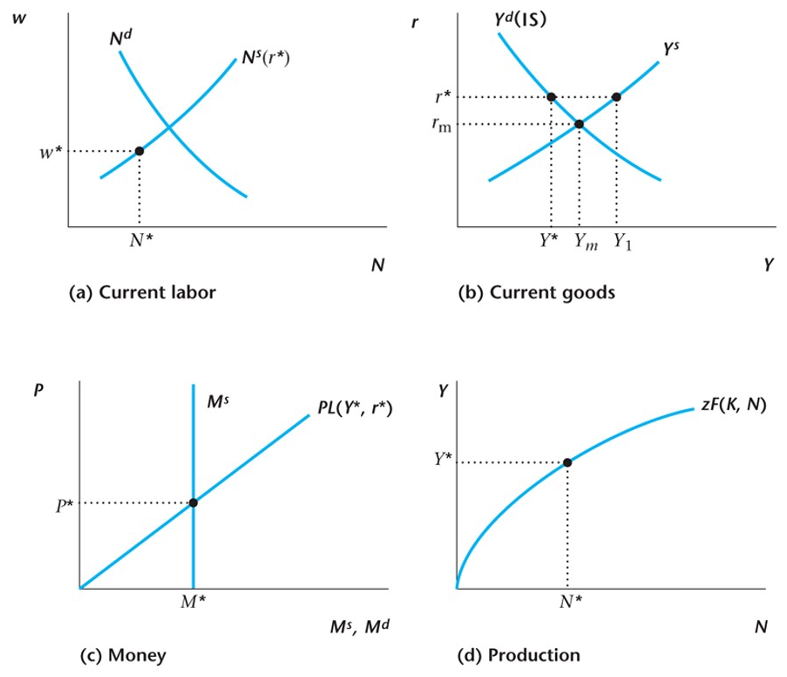
\includegraphics[scale=0.65]{Figures/W_Fig_14pt1.png}
\end{figure}
$r^*\rightarrow Y^d\rightarrow N\rightarrow w$, and given $Y$ and $r$, have $M$ and $P$
\end{frame}

\begin{frame}
\frametitle[alignment=center]{New Keynesian Model}
\begin{itemize}
\item Ok, so we broke our model a little via allowing the central bank, rather than the market, to choose $r$ (P doesn't move to clear markets, because sticky)
\bigskip
\item One way of thinking of this is that:
\begin{itemize}
\item Before, $Y^s=Y^d$ set $r$, and $N^s=N^d$ set $w$
\item Now, $r$ is set, $Y_d$ determines $Y$, and $Y$ determines $N^d$
\end{itemize}
\item In some sense, we replace the $Y^s$ curve to be horizontal (set by $r$) and the $N^d$ curve to be vertical (set by $Y$, which was set by $r$). 
\bigskip
\item One way to make sense of this is to have firms be making a little profit, so they're willing to supply at whatever (set) price there is (``monopolistic competition" can do this)
\bigskip
\item So what can govt do?
\end{itemize}
\end{frame}


\begin{frame}
\frametitle[alignment=center]{A Decrease in the Real Interest Rate in the NK Model}
\begin{figure}
\centering
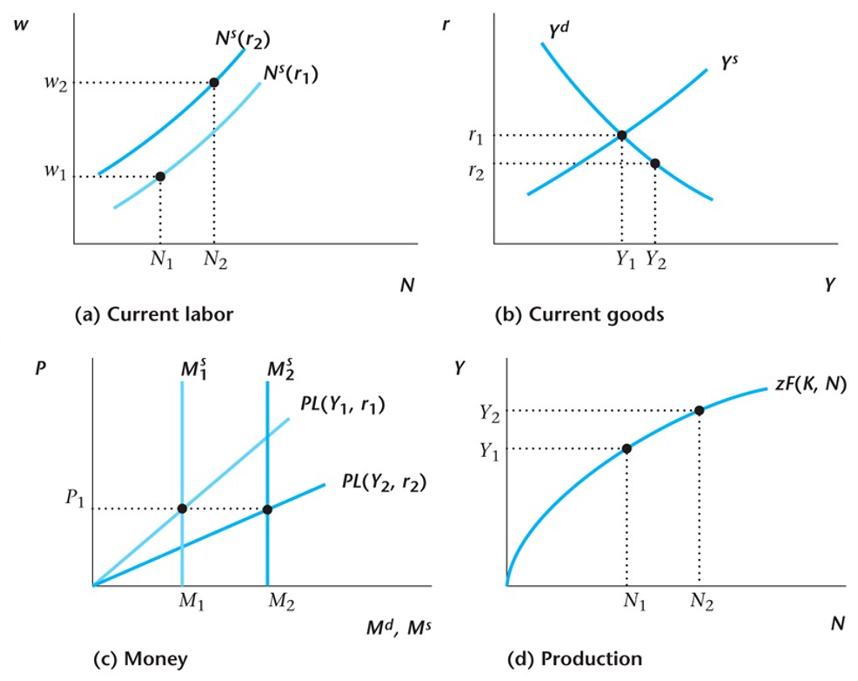
\includegraphics[scale=0.6]{Figures/W_Fig_14pt2.png}
\end{figure}
Two ways to describe what's happening here
\end{frame}

\begin{frame}
\frametitle[alignment=center]{A Decrease in the Real Interest Rate in the NK Model}
\begin{itemize}
\item Govt lowers $r$, which increases $Y$, which increases $N$ (but decreases $N^S$) and $M^d$, so $M^s$ must increase and $w$ decrease.  $N$ increased but $N^s$ decreased, raising wages
\bigskip
\item Or, money supply increases, which drives down interest rates ($M^s=M^d$).  As interest rates fall, demand rises, raising the real wage and employment
\bigskip
\item Flipped what we controlled: $r$ in the first case, $M$ in the second, but they're joined by $M^s=M^d$. 
\bigskip 
\item Money is no longer neutral (in the short run)
\bigskip
\item Note that in the long run, however, prices aren't fixed, and so we get back to our old real model
\end{itemize}
\end{frame}

\begin{frame}
\frametitle[alignment=center]{Government Stabilization}
\begin{itemize}
\item Now we have a model in which the government (central bank in this case) can affect the economy
\bigskip
\item Should the government try to ``stabilize" fluctuations in $Y$?
\bigskip
\item If prices are too high (or $r_1$ is too high so output gap), then govt can fix by setting right $r$ (or right $P$ via $M^s$)
\bigskip
\item Alternatively, govt can increase demand (increasing r, so economy not in disequilibrium)
\end{itemize}
\end{frame}

\begin{frame}
\frametitle[alignment=center]{Monetary Policy can ``fix" }
\begin{figure}
\centering
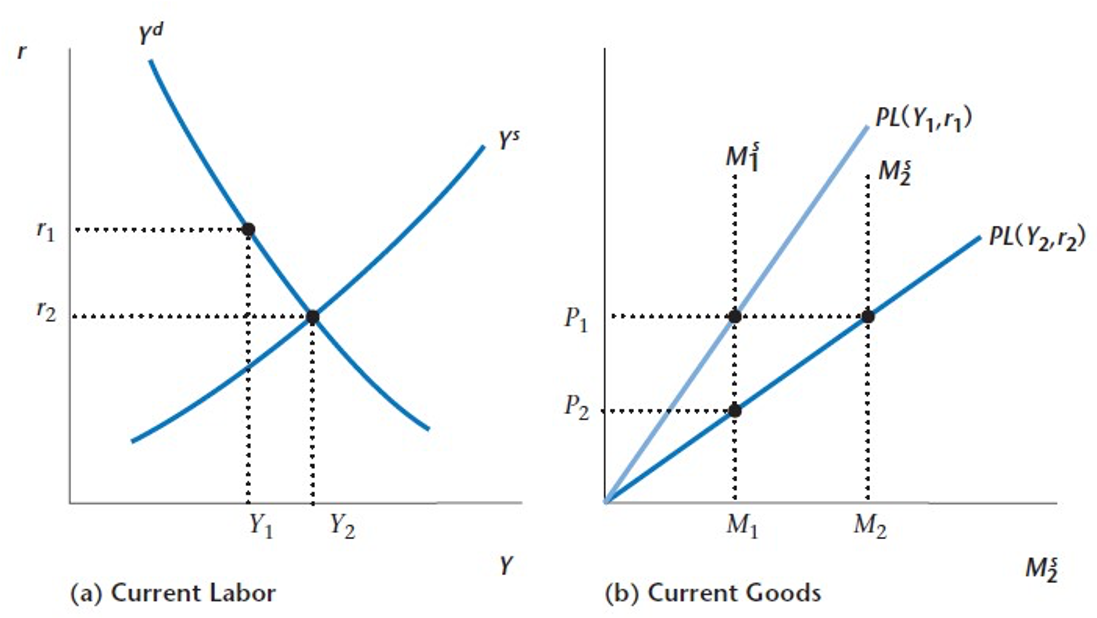
\includegraphics[scale=0.65]{Figures/W_Fig_14pt3.png}
\end{figure}
If prices too high, could wait for them to drift down over time, or fix by choosing right $M$ (or $r$) in short run
\end{frame}


\begin{frame}
\frametitle[alignment=center]{Fiscal Policy can ``fix" }
\begin{figure}
\centering
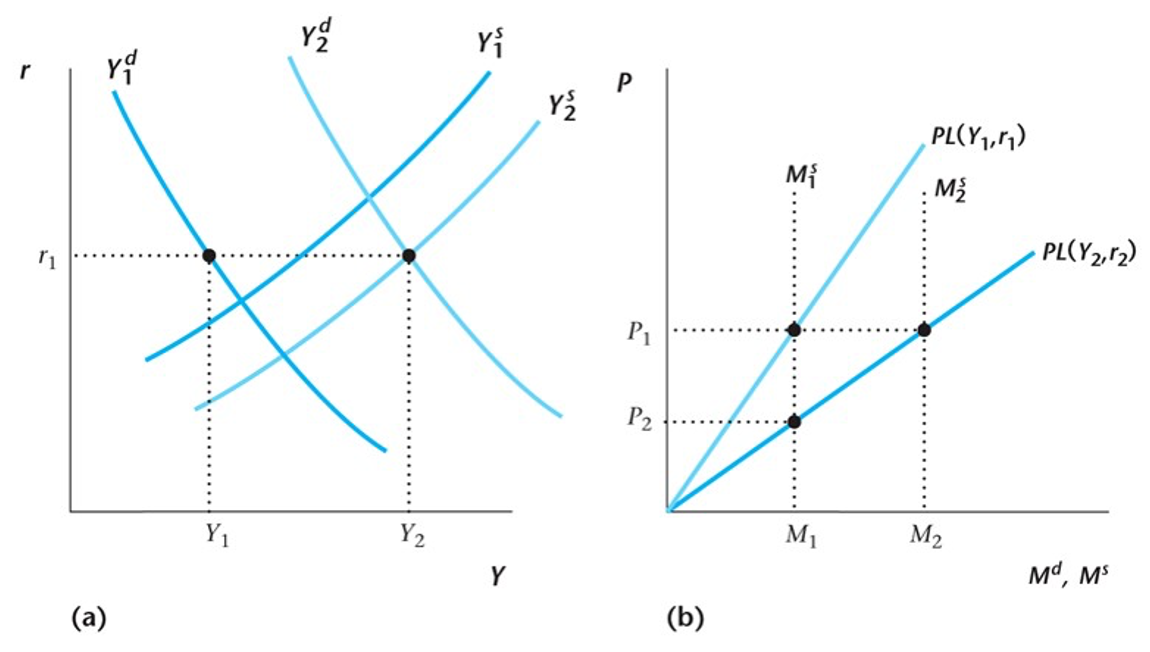
\includegraphics[scale=0.65]{Figures/W_Fig_14pt4.png}
\end{figure}
If $r$ too high, can shift out demand until markets clear
\end{frame}

\begin{frame}
\frametitle[alignment=center]{Comparing Fixes }
\begin{itemize}
\item Both solutions start with observation: there is an ``output gap" because $r$ artificially high
\bigskip
\item Monetary policy fixes this by increasing $M$/lowering $r$
\bigskip
\item Fiscal policy fixes this by increasing $Yd$ until $r$ is the equilibrium (r fixed)
\bigskip
\item Fiscal policy is entire $Y^d$ increase (Ch. 11), so $C$ and $I$ don't increase, where for monetary, $C$ and $I$ increase 
\bigskip
\item Okay, we have the theory--how is the data on the NK model?
\end{itemize}
\end{frame}


\begin{frame}
\frametitle[alignment=center]{Can we replicate the data? }
\begin{itemize}
\item Assume central bank wants to minimize output gap (make sure $Y^d=Y^s$)
\bigskip
\item Now take a positive and persistent TFP shock to $z$, which shifts out $Y^d$ and $Y^s$, $Y^s$ more
\bigskip
\item But if $r$ doesn't move to clear interest rates, then output gap--interest rates too low
\bigskip
\item Interest rates should fall
\bigskip
\item Monetary policy fixes this by increasing $M$/lowering $r$
\bigskip
\item Fiscal policy fixes this by increasing $Yd$ until $r$ is the equilibrium (r fixed)
\bigskip
\item Fiscal policy is entire $Y^d$ increase (Ch. 11), so $C$ and $I$ don't increase, where for monetary, $C$ and $I$ increase 
\bigskip
\item Okay, we have the theory--how is the data on the NK model?
\end{itemize}
\end{frame}


\begin{frame}
\frametitle[alignment=center]{Persistent TFP Increase}
\begin{figure}
\centering
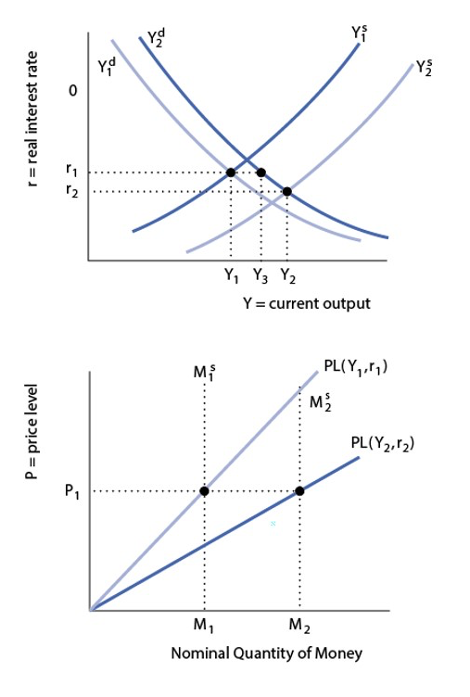
\includegraphics[scale=0.65]{Figures/W_Fig_14pt5.png}
\end{figure}
$Y^s$ and $Y^d$ increase, and output gap increases, so central bank should lower $r$ (increase $M$) and clear markets
\end{frame}

\begin{frame}
\frametitle[alignment=center]{Can we replicate the data? }
\begin{itemize}
\item If the central bank is clearing markets, we'll look like a market-clearing model
\bigskip
\item E.g. same as our real model!
\bigskip
\item Can't necessarily tell these apart
\end{itemize}
\end{frame}

\begin{frame}
\frametitle[alignment=center]{The Zero Lower Bound }
\begin{itemize}
\item As discussed before, we can't cause $r$ to be lower than 0 (otherwise people just use money)
\bigskip
\item Before, central bank was switching $M$ and $B$ in open market operations--now same thing
\bigskip
\item Let's think about a shock to credit frictions
\end{itemize}
\end{frame}


\begin{frame}
\frametitle[alignment=center]{The ``Liquidity Trap"}
\begin{figure}
\centering
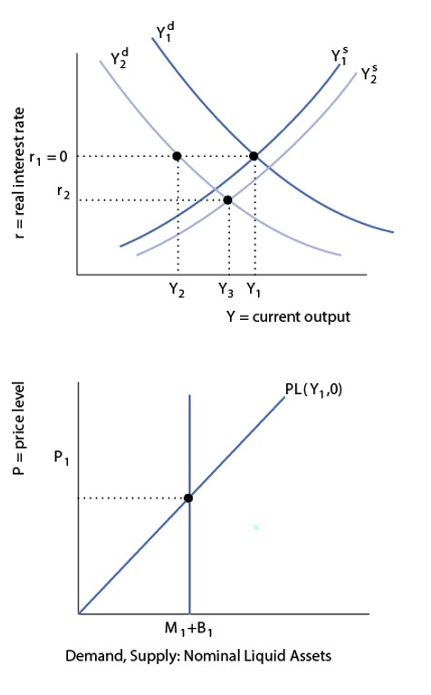
\includegraphics[scale=0.62]{Figures/W_Fig_14pt6.png}
\end{figure}
Credit frictions decreases $Y^d$, but $r$ can't fall, so $Y$ falls much more. $L(Y,0)$ means $M^s=M+B$
\end{frame}

\begin{frame}
\frametitle[alignment=center]{The Taylor Rule}
\begin{itemize}
\item Some suggest rules-based policy for $r$ might be useful
\bigskip
\item For instance, if $Y$ is GDP, $Y^*$ is market-clearing output, $i$ is inflation, $i^*$ is target inflation, might get:
$$R=2+\beta_2(i-i^*)-\beta_1(Y-Y^*)$$
\item Where $\beta_1$ and $\beta_2$ are some weights we put on deviations 
\bigskip
\item When output is too low, then lower interest rate, when inflation too high, raise it
\bigskip
\item Puts a balancing of inflation and market-clearing motivations into a single, expected tradeoff
\bigskip
\item Let's see how it does!
\end{itemize}
\end{frame}



\begin{frame}
\frametitle[alignment=center]{Taylor Rule Explains 1988-2007 pretty well!}
\begin{figure}
\centering
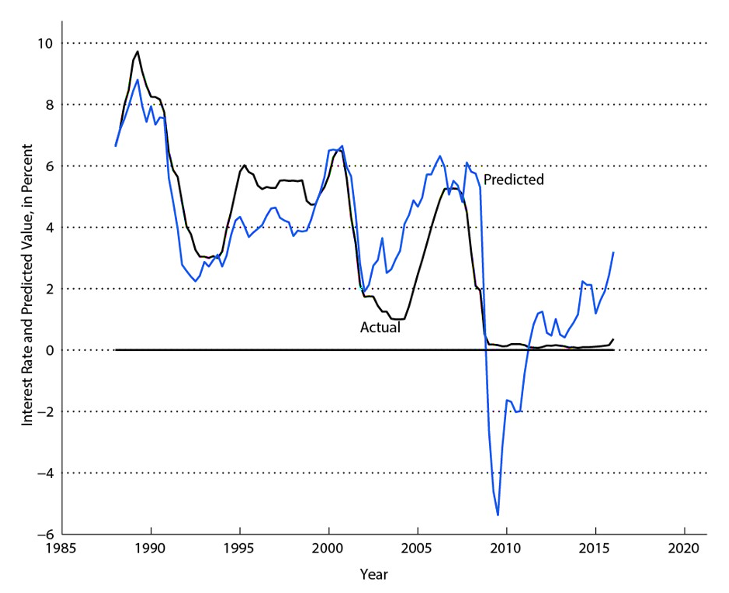
\includegraphics[scale=0.65]{Figures/W_Fig_14pt7.png}
\end{figure}
Williamson Taylor Rule
\end{frame}

\begin{frame}
\frametitle[alignment=center]{Taylor Rule (1988-2016)}
\begin{figure}
\centering
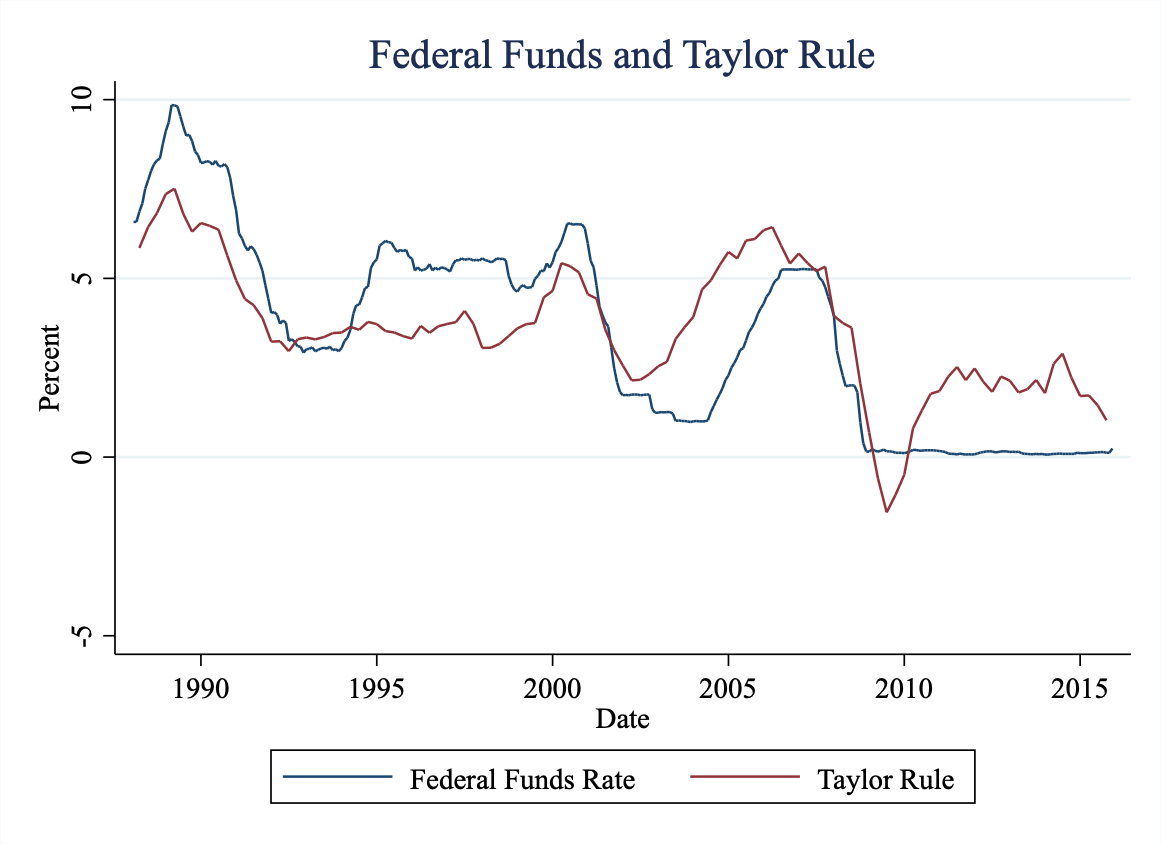
\includegraphics[scale=0.25]{Figures/FedFunds1.png}
\end{figure}
Our version is quarterly, but similar
\end{frame}

\begin{frame}
\frametitle[alignment=center]{Taylor Rule (1988-2022)}
\begin{figure}
\centering
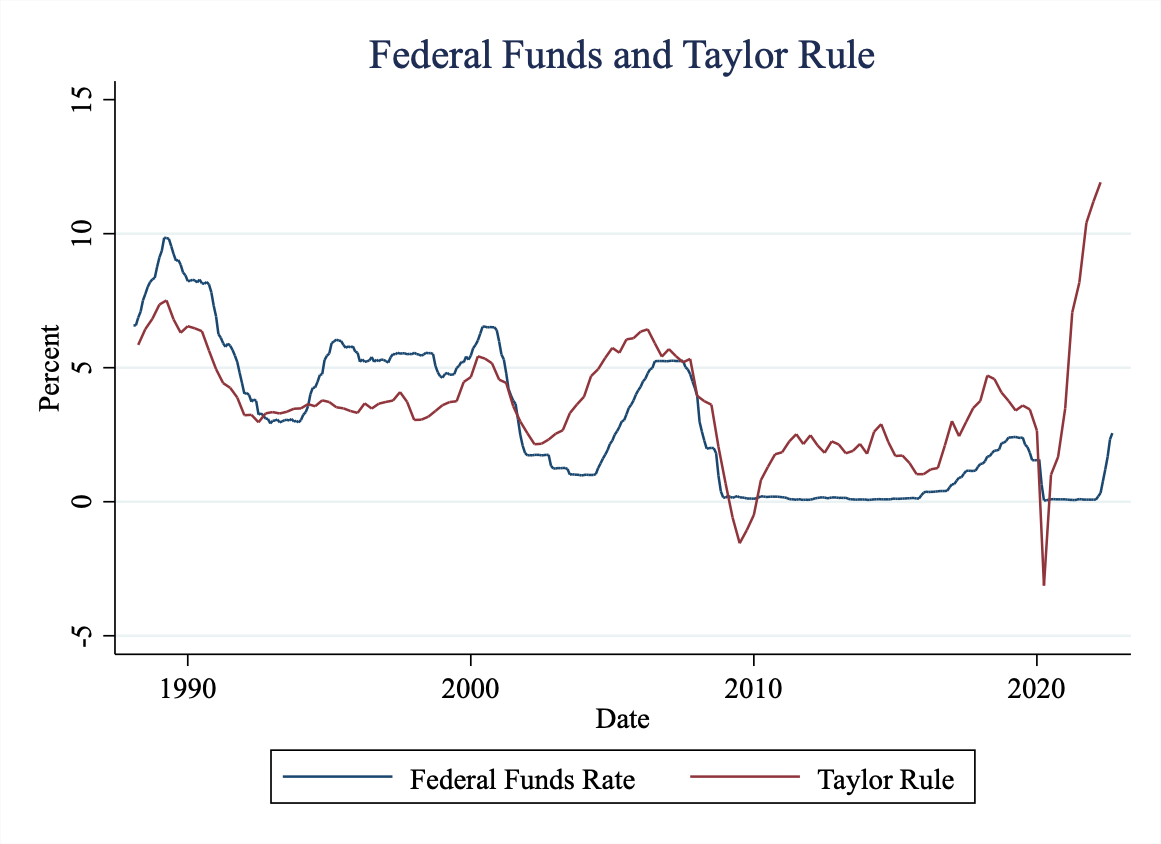
\includegraphics[scale=0.25]{Figures/FedFunds2.png}
\end{figure}
Seems like history demands \emph{way} higher interest rates!
\end{frame}

\begin{frame}
\frametitle[alignment=center]{Taylor Rule (1954-2022)}
\begin{figure}
\centering
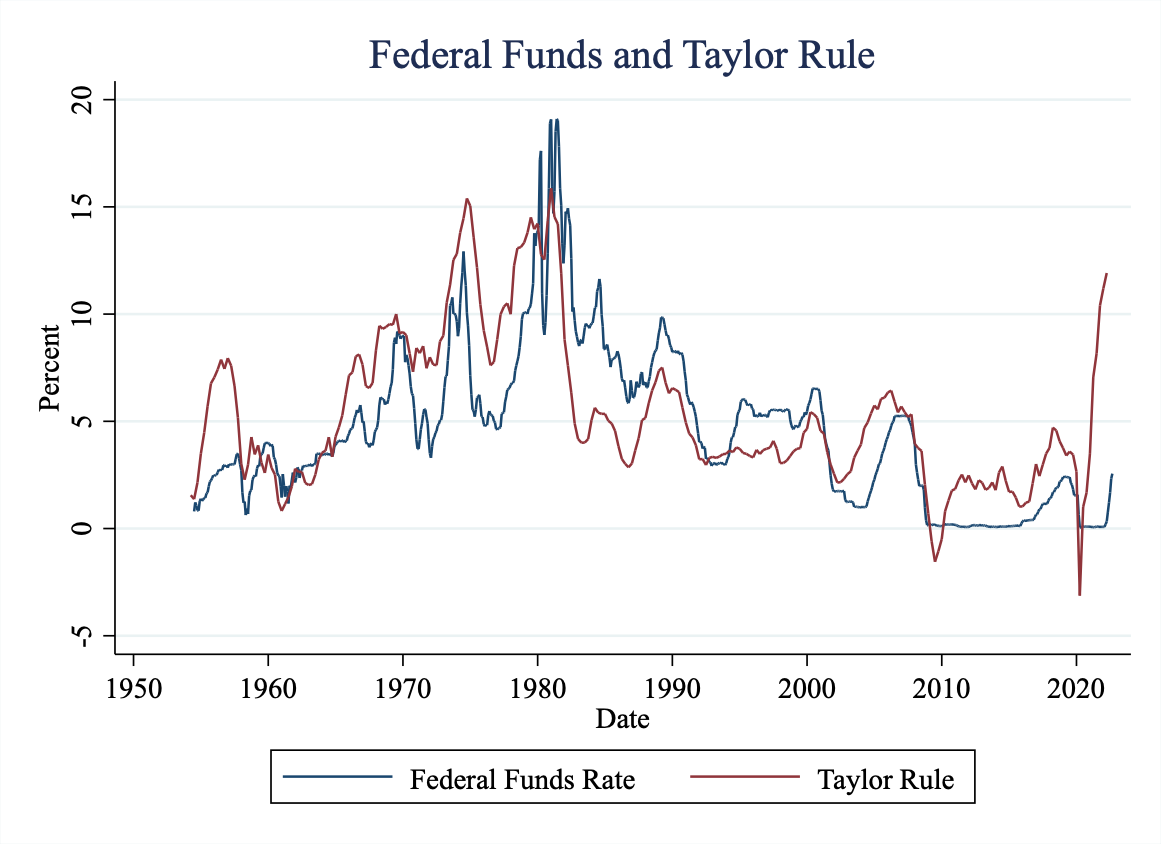
\includegraphics[scale=0.25]{Figures/FedFunds3.png}
\end{figure}
When Taylor Rule higher than FFR, expect inflation!
\end{frame}

\begin{frame}
\frametitle[alignment=center]{Keynesian Criticisms}
\begin{itemize}
\item NK models simply assume sticky prices
\bigskip
\item But why are they sticky?  And how sticky are they?
\bigskip
\item Similarly wages:  why don't wages drop if there are unemployed people?
\end{itemize}
\end{frame}


\end{document}